\documentclass[12pt]{article}
\usepackage{subcaption}
\usepackage{graphicx}

\usepackage{pifont,amssymb} % for the symbols
\usepackage[shortlabels]{enumitem}

\newlist{answerlist}{enumerate}{2}
\setlist[answerlist]{label={\arabic*.\makebox[0pt][r]{\noexpand\emptysquare\hspace{2em}}},ref=\alph*}

\newcommand{\emptysquare}{$\square$}
\newcommand{\checkedsquare}{\makebox[0pt][l]{\raisebox{1pt}[0pt][0pt]{\large\hspace{1pt}\cmark}}$\square$}
\newcommand{\cmark}{\ding{51}}%
\newcommand{\correctanswer}{{\renewcommand{\emptysquare}{\checkedsquare}\item\leavevmode}}

\title{Source Carriage Assembly Instructions}
\author{Ryan Bayes}
\date{\today}

\begin{document}
\maketitle
\section{Introduction}

This document describes the cleaning, handling, and assembly of the
elements of the source carriage. This includes the source pivot, the
UFO housing, and the source connector (top screw and nut). These parts
are not very well documented elsewhere, but they are key to the
assembly of the calibration hardware system. These pieces are permanently
fixed to the umbilical

\section{Part Descriptions}

\subsection{Source Pivot}
The source pivot is the upper most element of the source
assembly. This consists of a nut that fits snugly to the umbilical
with a rotating collar (the pivot) intended to provide a tie-off point
for the central rope. The pivot attaches to a pully flange, which
supports the fixed side rope pulleys, via a pin joint. The assembly
supports lower elements of the source via a pair of brackets. Design
drawings of the completed assembly are shown in Fig.\ref{fig:pivot}.

\begin{figure}
  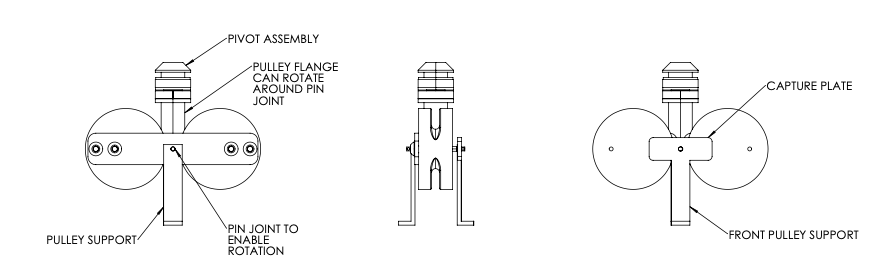
\includegraphics[width=\textwidth]{SourcePivot}
  \caption{Source pivot and side rope pulleys}
  \label{fig:pivot}
\end{figure}

\subsection{UFO housing}
The umbilical flasher object (UFO) was intended to provide information
of the source location to the detector independent of the manipulator
system. As the central boards are not ready at this, this
functionality will not be available. However the housing for the UFO
will be used for the source assembly. The housing consists of a top
plate, an acrylic cylinder and a steel cylinder. The three pieces are
held together using long screws that connect the top plate to the
steel cylinder through conduits in the acrylic housing. The umbilical
is clamped into the UFO housing using a series of pressure plates that
are secured to the top plate. The source pivot also attaches to the
top plate of the UFO. Design drawings for the UFO cylinder and plate are
shown in Fig.\ref{fig:UFO}.

\begin{figure}
  \begin{center}
  \begin{subfigure}{0.4\textwidth}
    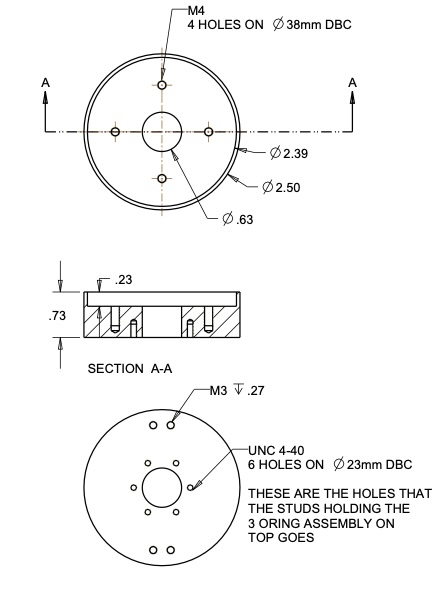
\includegraphics[width=\textwidth]{UFOTopPlate}
    \caption{Top plate}
  \end{subfigure}
  \begin{subfigure}{0.4\textwidth}
    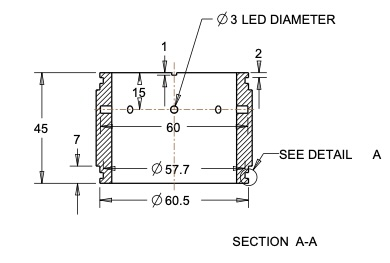
\includegraphics[width=\textwidth]{UFOAcrylicHousing}
    \caption{Acrylic cylinder}
   \end{subfigure}
  \begin{subfigure}{0.4\textwidth}
    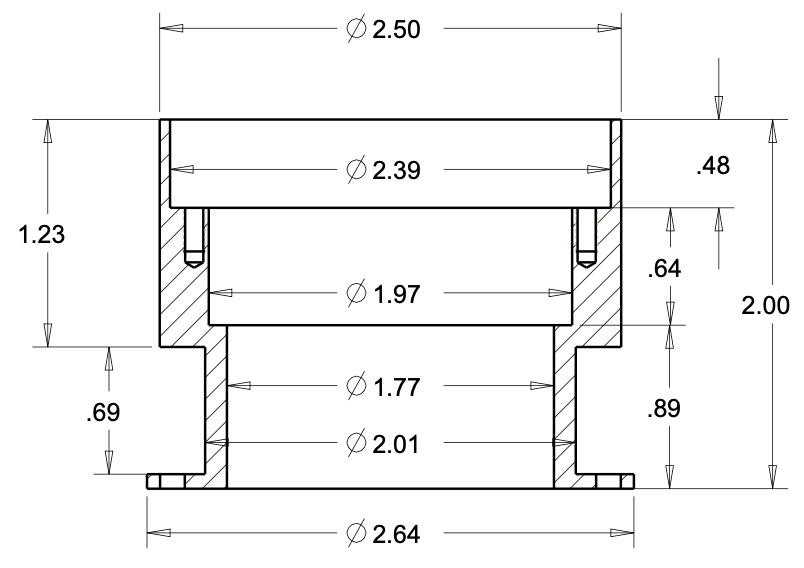
\includegraphics[width=\textwidth]{UFOSteelCylinder}
    \caption{Steel Cylinder}
  \end{subfigure}
  \begin{subfigure}{0.4\textwidth}
    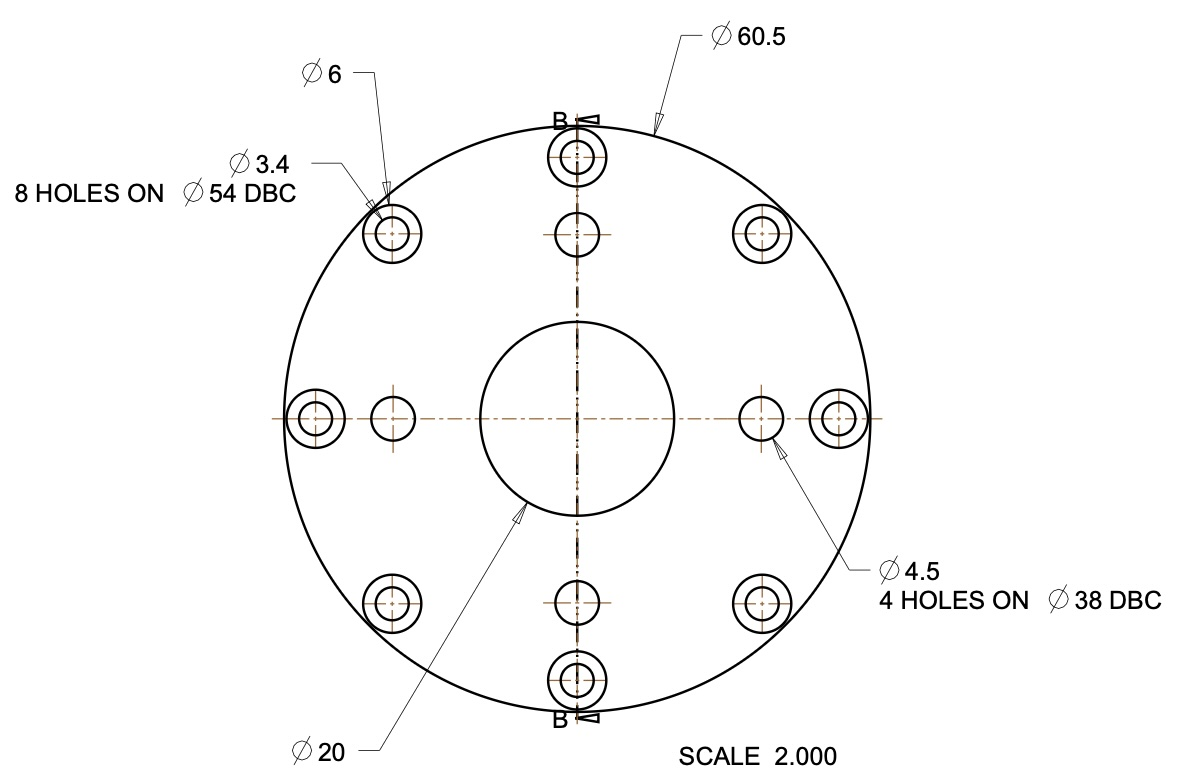
\includegraphics[width=\textwidth]{UFOBottomPlate}
    \caption{Acrylic Bottom Plate}
  \end{subfigure}
  \caption{Umbilical flasher object housing}
  \label{fig:UFO}
  \end{center}
\end{figure}

\subsection{Source Connector}
The last permainent installation on the umbilical is the source
connector. This consists of a barrel with a left handed screw thread
on one end which is capped by a feed through which couples the optical
fibre in the umbilical to the quartz rod in the Laserball (which
terminates in a right hand thread source connector). The source
connector and a source (either the Laserball or the AmBe source) are
held together with a nut that contains corresponding threads (left
handed on the top half, right handed on the bottom half) such that the
umbilical side and the source side can be drawn together simply by
turning the nut in a clockwise direction while the umbilical and
source remain stationary. Alignment rods installed on the source
connector plates ensure the source and umbilical alignment through
source installation. A detail of the source connector is shown in
Fig.\ref{fig:SC} with a picture of the assembled source connector in
Fig.\ref{fig:SCP}.

\begin{figure}
  \begin{center}
\begin{subfigure}{0.4\textwidth}
  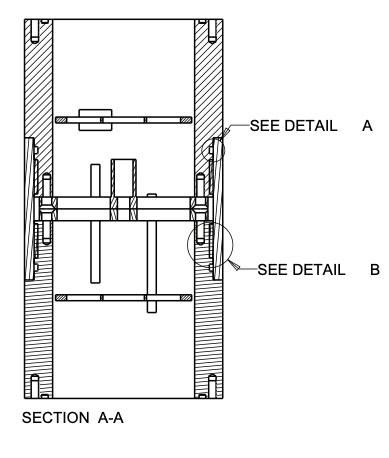
\includegraphics[width=\textwidth]{SourceConnectorSection}
  \caption{Source connector detailed drawing}
  \label{fig:SC}
\end{subfigure}
\begin{subfigure}{0.4\textwidth}
  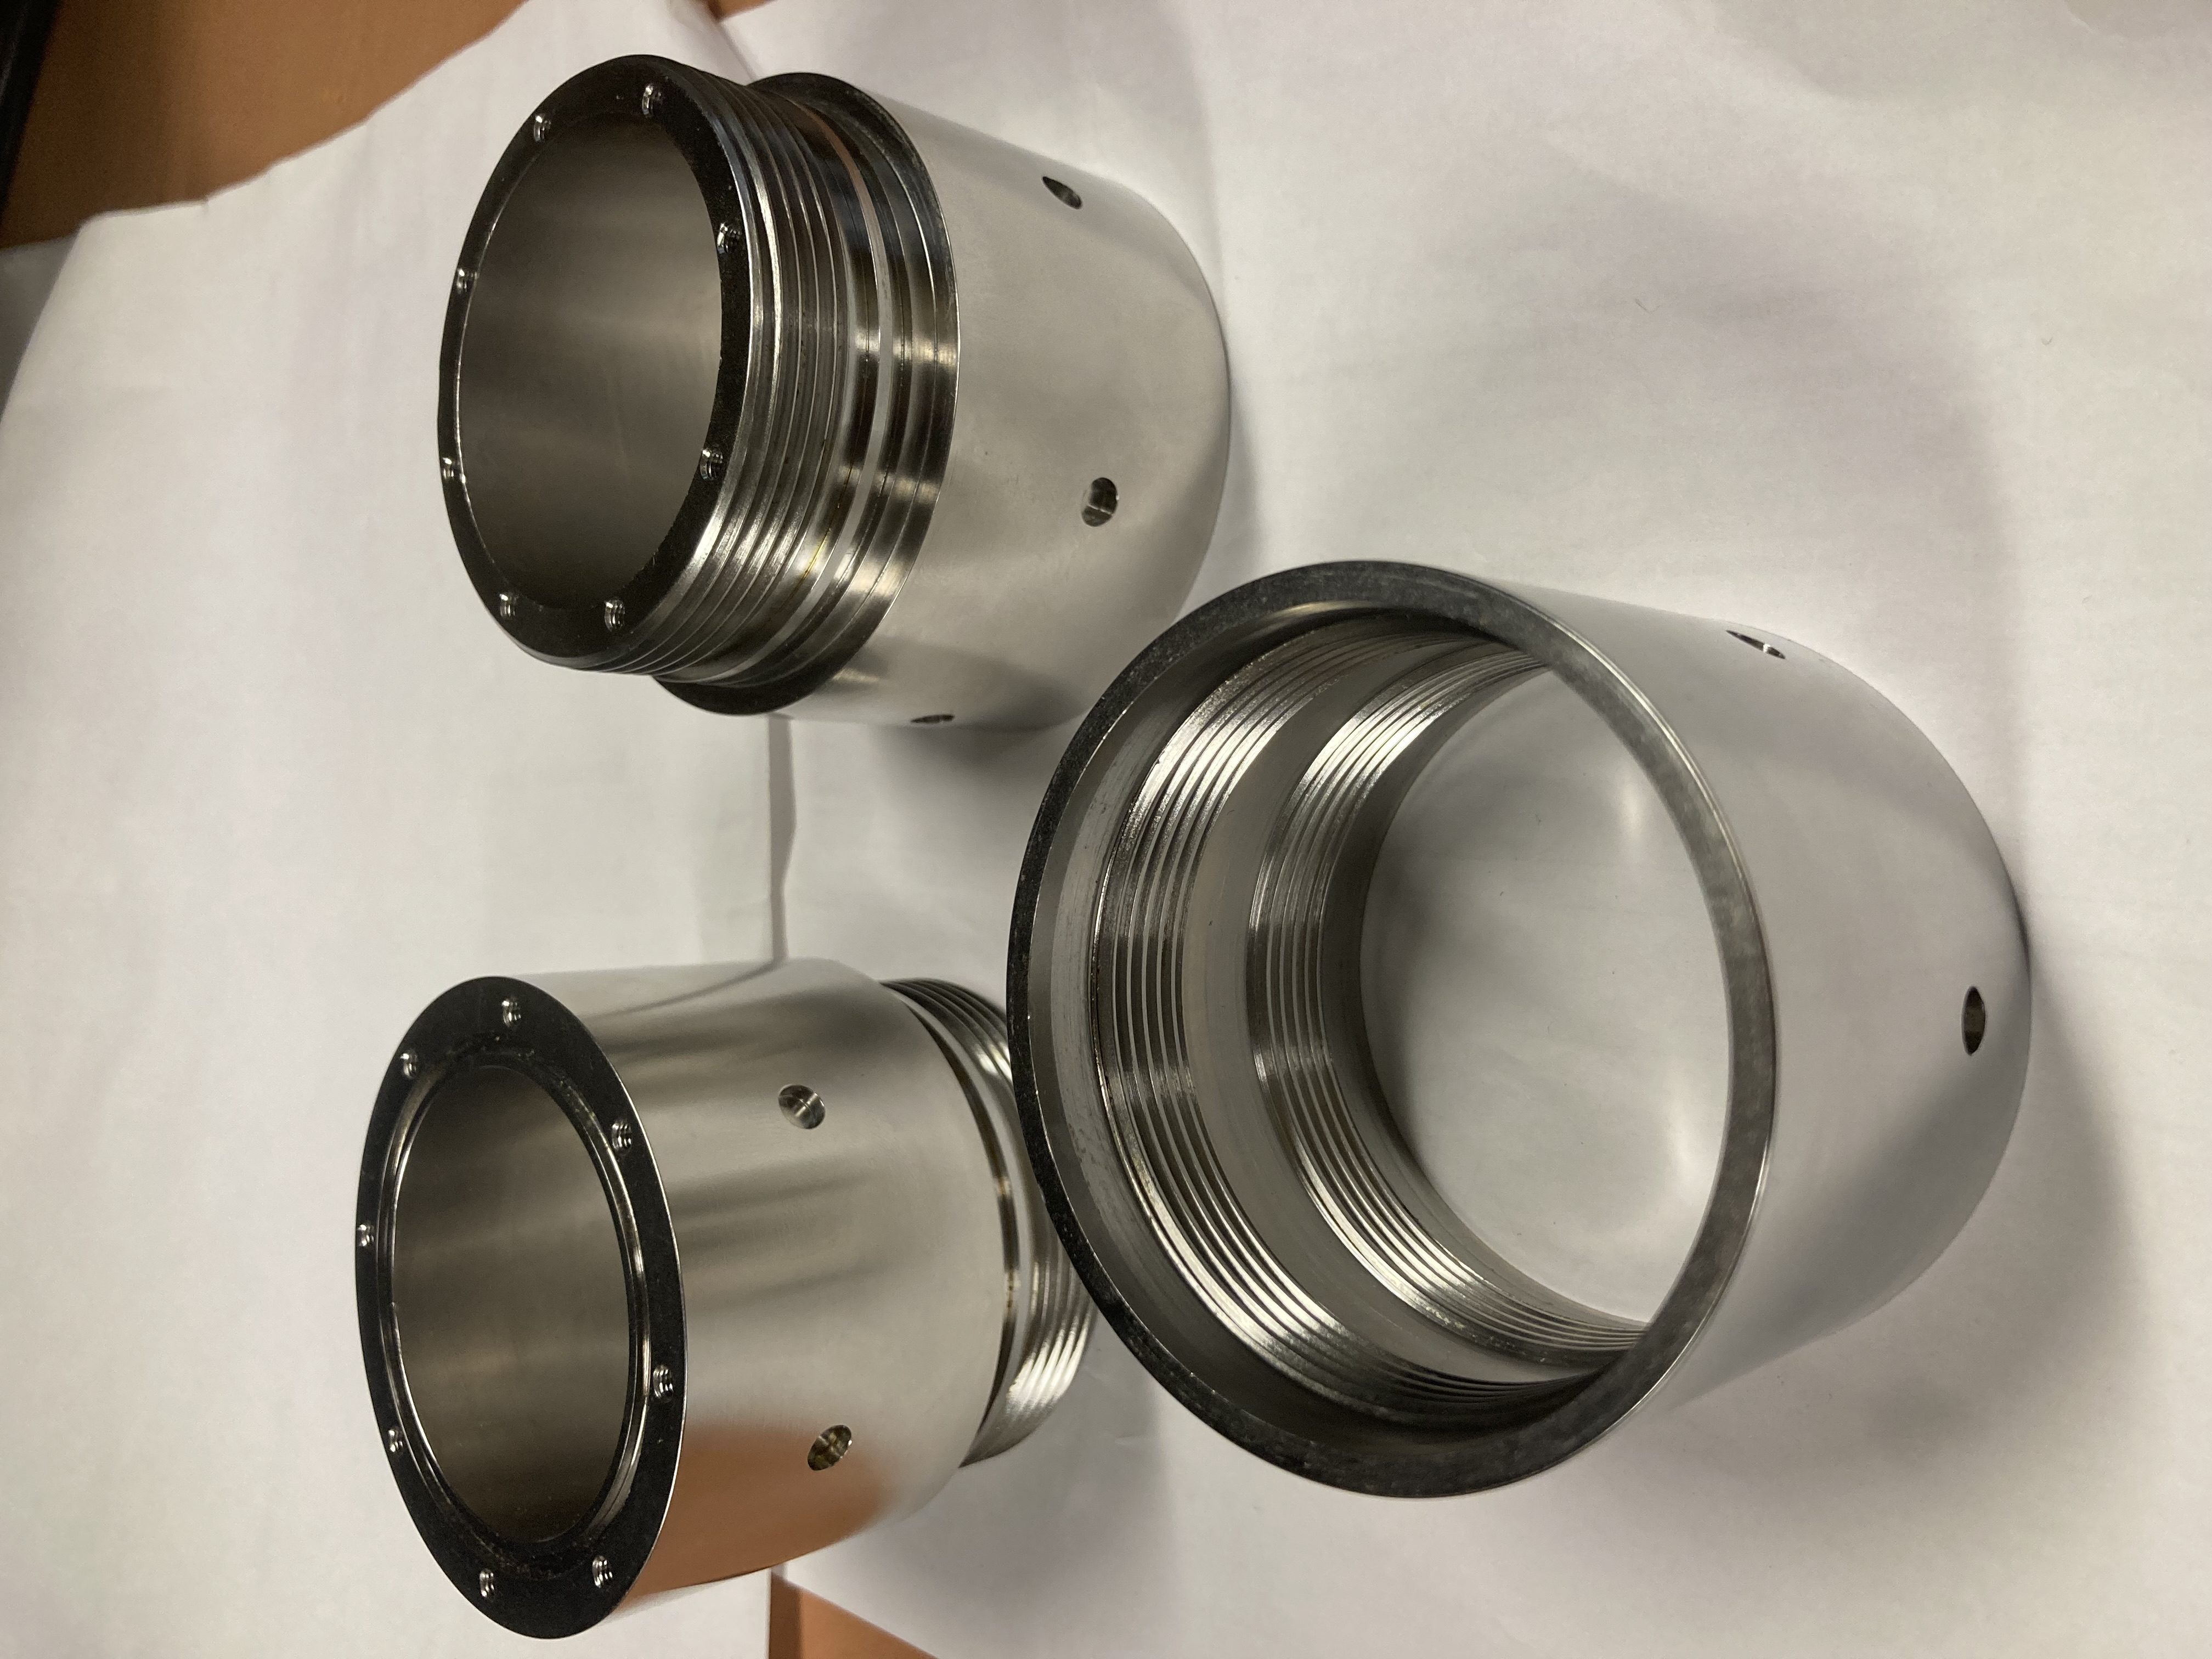
\includegraphics[height=\textwidth,angle=270]{IMG_5710}
  \caption{Source connector in hand}
  \label{fig:SCP}
\end{subfigure}
\end{center}
\caption{Source connector.}
\end{figure}

\section{Cleaning, Handling and Assembly}

All of the components of this assembly are stainless steel an
acrylic. It is assumed that the majority of cleaning for the various
components will be completed using ultra-sonic cleaning. The steps for
ultra-sonic cleaning involves
\begin{itemize}
\item Placing all of the items in the cleaner basket.
\item Fill the US cleaner volume with UPW
\item Add NuClean to the volume with a 1:50 concentration (NuClean to UPW)
\item Run the cleaner through a 60 minute cycle. This involves heating
  the volume to 60 degrees celcius, while applying ultra sonic
  frequencies.
\item Drain the cleaner with the components in place. Refill the
  cleaner volume with UPW. Run the cleaner for 30 minutes for a first
  rinse.
\item Drain the cleaner with the components in place. Refill the
  cleaner volume with UPW and run the cleaner for 60 minutes for a
  second rinse.
\item Drain the cleaner and remove the components from the ultra sonic cleaner
\item Dry all of the components with lint free cloths.
\item Place the components in plastic bags as appropriate.
\end{itemize}
Nitrile gloves must be worn at all times when handling the components
before, during and after the cleaning procedure.

At the present time, all of the parts for the source pivot assembly
are underground, the parts of the source connector and UFO housing are
on surface and were cleaned as part of the Laserball preparation, and
a second source connector assembly (for the AmBe source) is also on
surface and still to be cleaned. The parts that remain on surface are
intended to be taken underground by hand after triple bagging all of
the components. An additional plastic bag should be added for drift
travel, to be removed immediately upon entering the lab. The next most
outer bag should be removed before the assembly is moved to the
control room. The second to last layer should be wiped down with a
lint free cloth and UPW before the assemblage is moved to the DCR.

Assembly of the source carriage requires the cleaned and
installed umbilical and central rope. It may be reasonable to conduct a
limited pre-assembly of the source pivot well before the final
installation. Assembly consists of
\begin{answerlist}
\item Wet the bottom metre of umbilical with LAB
\item Pre-wet all of the screws with LAB
\item Install o-rings on the UFO acrylic cylinder, the source
  connector top and bottom surfaces.
\item Threading the umbilical through the pivot
\item Thread the umbilical through the pressure plates with appropriate o-rings.
\item Thread the umbilical through the top plate of the UFO.
\item Ensuring that there is a surplus of umbilical below the top
  plate of the UFO run the umbilical through the UFO acrylic, steel plate and
  stainless steel cylinder, and the upper source connector body.
\item Couple the end of the fibre bundle to the source connector plate.
\item Secure the source connector plate to the source upper source
  connector body with 8 m2 screws.
\item Fasten the UFO bottom plate to the top of the UFO steel cylinder.
\item Align the acrylic cylinder between the top section and the UFO
  plate and thread the support rods into the top plate. Once the
  threaded rod is secured, tighten the UFO assembly together using the
  appropriate nuts.
\item Fasten the UFO steel cylinder to the top of the upper source
  connector with 8 m3 cap screws.
\item Tighten the presure plates against the top of the UFO assembly
  using four M3 screws.
\item Secure the source pivot pully support plates to the UFO assembly.
\item Tie the central rope to the rotating collar on the pivot assembly.
\end{answerlist}

Questions:
\begin{itemize}
\item Do we have the pressure plates with the Laserball? Are these plates elsewhere?
\item Does the source pivot clamp down on the umbilical?
\item Is there enough room to turn a wrench to secure the threaded rod?
\item Is the fibre bundle assembly procedure written elsewhere?
\end{itemize}

\section{Usage}
Once the source connector has been assembled with the umbilical,
sources can be exchanged with little difficult. At this time only two
sources are planned; the Laserball and the AmBe source. Installation
of the laserball is the more sensitive of the two. The steps for this
involve two people equipped with standard PPE and nitrile
gloves. Assuming the source connector is exposed below the bellows
gate valve;
\begin{answerlist}
\item Remove the source connector end of the source from it's storage bag (leave the diffuser inside the bag).
\item Match the source connector to the umbilical source connector with the nut between them using the guide studs to locate the relative location of the two plates.
\item With the help of a collegue push the two source connector ends together until they meet the threads of the nut, then hold the source connector ends in place while turning the nut clockwise.
  \begin{itemize}
  \item If the nut does not thread easily, the nut will have to be flipped.
  \item If there is any resistance before the nut is completely threaded stop, check the orientation of guide studs and the alignment of the quartz rod before starting over.
  \end{itemize}
\item With the nut completely threaded, the complete source assembly should be snugly in place. Test by applying a little more force in the clockwise direction.
\item Remove the bag from the diffuser flask. Raise the source into the URM.
\end{answerlist}
These steps will be identical for the AmBe source except there will be be no guid rods to align as there is no optical rod to match.

\begin{thebibliography}{99}
\item[PulleyDesign] Mitchel Baker, ``Pulley Assembly July 9, 2021'', private communication
\item[SammyLB] Sammy Valder, ``The SNO+ Laserball Source for Scintillator Phase'', DocDB 7202
\item[KrausSC] Carsten Kraus, ``The Source Connector'', DocDB 
  
\end{thebibliography}

\end{document}
